\clearpage

\section{SuperK MC templates}
\label{sec:mc_templates}

The nominal SuperK MC templates
are shown in Figs. \ref{fig:etrue_ereco_templates:numu}-\ref{fig:etrue_ereco_templates:oscnue}.
They are shown in the binning used for the analysis, which is
84 true energy bins:
\begin{itemize}
\item   6 50-MeV bins from 0-0.3 GeV; 
\item   28 25-MeV bins from 0.3-1 GeV; 
\item   40 50-MeV bins from 1-3 GeV; 
\item   5 100-MeV bin from 3-3.5 GeV; 
\item   1 bin from 3.5-4 GeV; 
\item   1 bin from 4-5 GeV; 
\item   1 bin from 5-7 GeV; 
\item   1 bin from 7-10 GeV;
\item   1 bin from 10-30 GeV,
\end{itemize}
and 73 reconstructed energy bins:
\begin{itemize}
\item   60 50-MeV bins from 0-3 GeV; 
\item   4 250-MeV bins from 3-4 GeV; 
\item   4 500-MeV bins from 4-6 GeV; 
\item   4 1000-MeV bins from 6-10 GeV;
\item   1 bin from 10-30 GeV.
\end{itemize}

%
% Figs for \subsection{SuperK MC templates in the chosen binning}
%

\begin{figure*}[htb]
\center
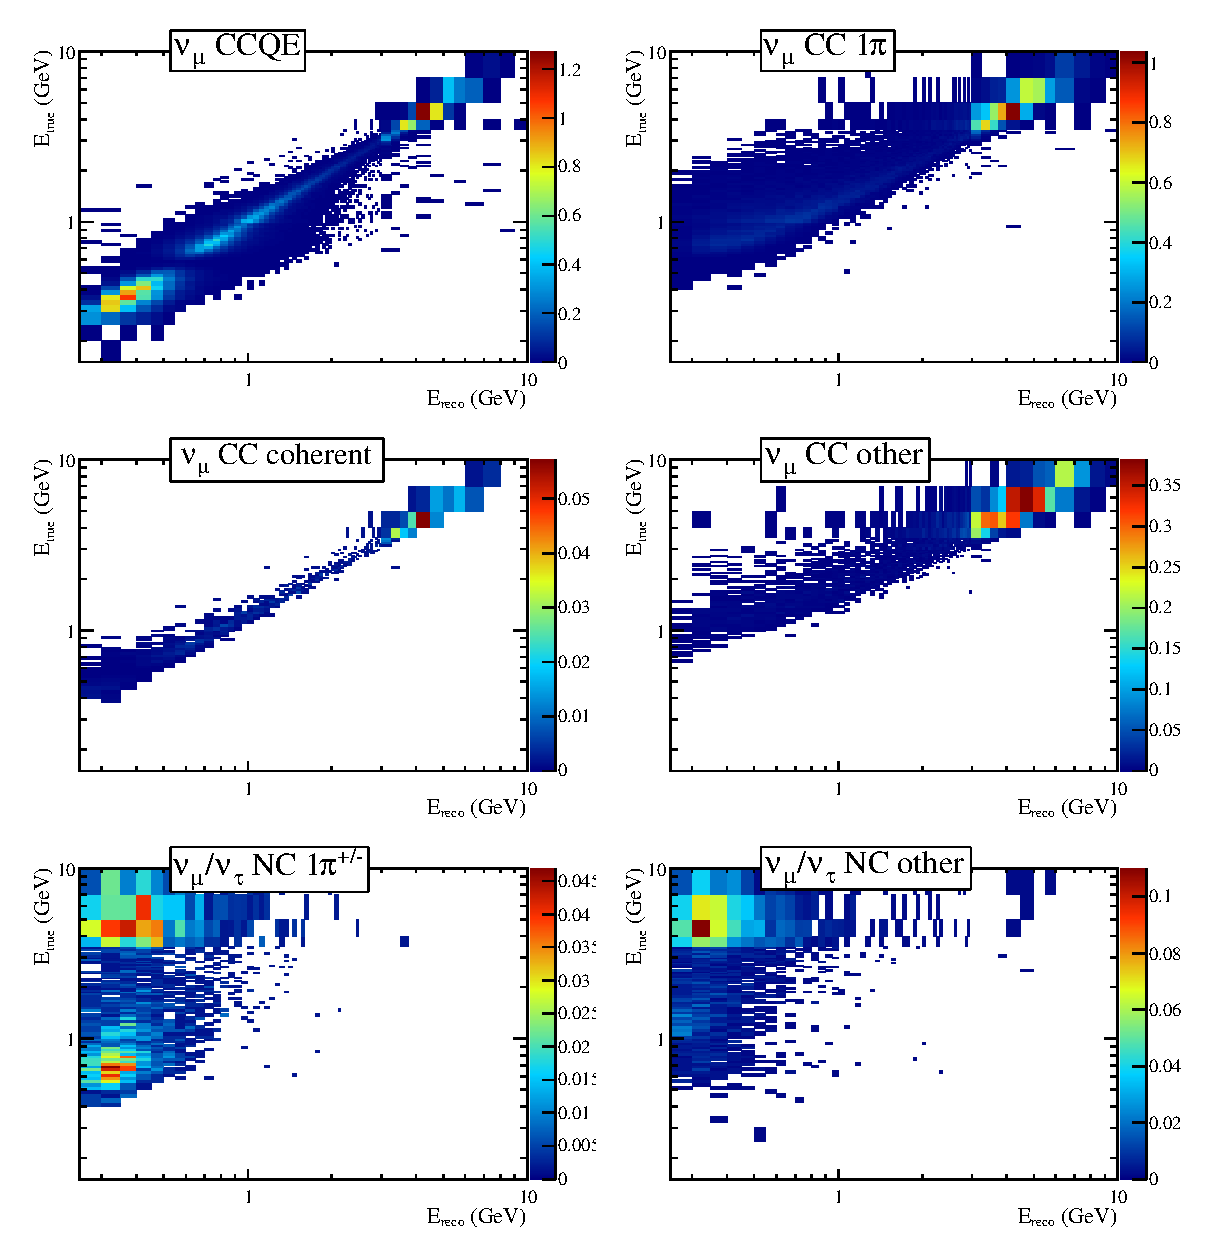
\includegraphics[width=35pc]{../images/templates/mc_template_0}
\caption{
  Nominal ($E_{t}$, $E_{r}$) 1-ring $\mu$-like MC templates. 
  The templates are shown for
  $\nu_{\mu}$ CCQE
  $\nu_{\mu}$ CC1$\pi$, 
  $\nu_{\mu}$ CC coherent, 
  $\nu_{\mu}$ CC other, 
  $\nu_{\mu}$ NC1$\pi^{\pm}$, 
  $\nu_{\mu}$ NC other.
}
\label{fig:etrue_ereco_templates:numu}
\end{figure*}

\begin{figure*}[htb]
\center
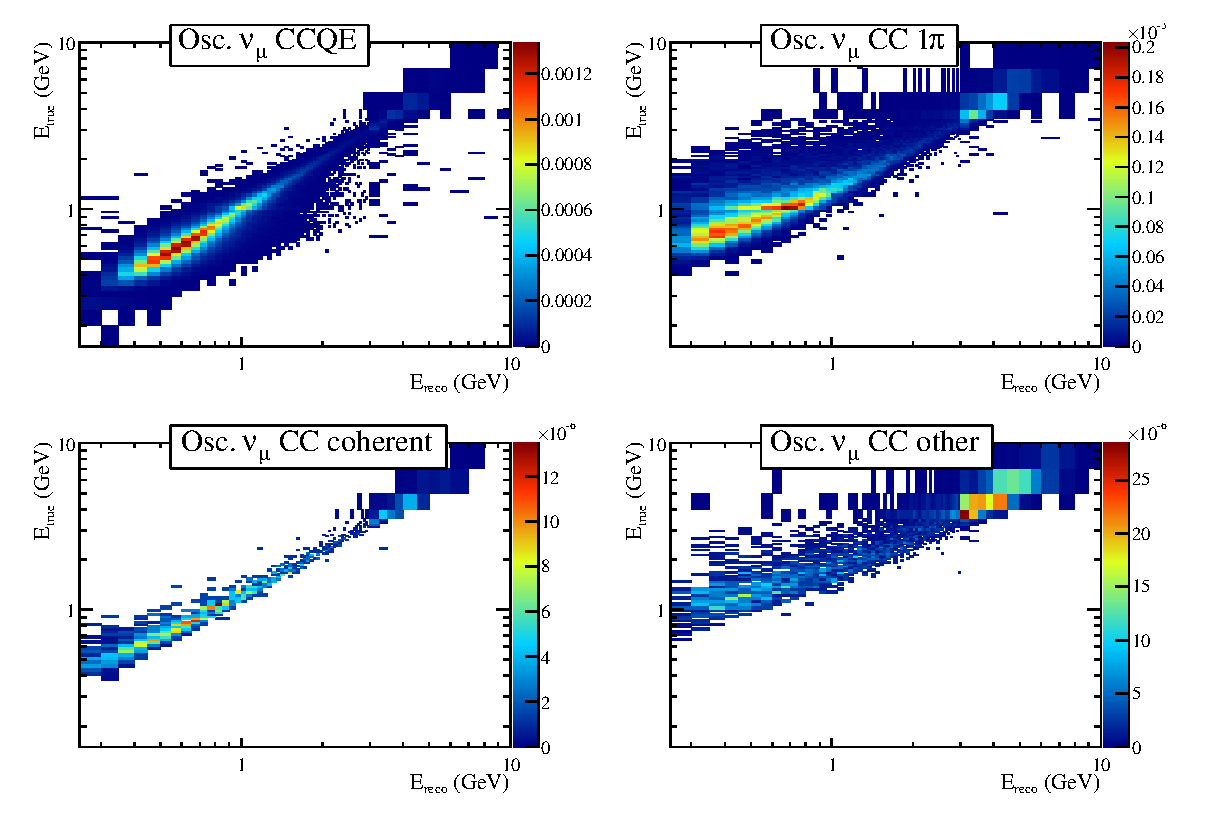
\includegraphics[width=35pc]{../images/templates/mc_template_1}
\caption{
  Nominal ($E_{t}$, $E_{r}$) 1-ring $\mu$-like MC templates. 
  The templates are shown for
  osc. $\nu_{\mu}$ CCQE, 
  osc. $\nu_{\mu}$ CC1$\pi$,
  osc. $\nu_{\mu}$ CC coherent and
  osc. $\nu_{\mu}$ CC other.
}
\label{fig:etrue_ereco_templates:oscnumu}
\end{figure*}

\begin{figure*}[htb]
\center
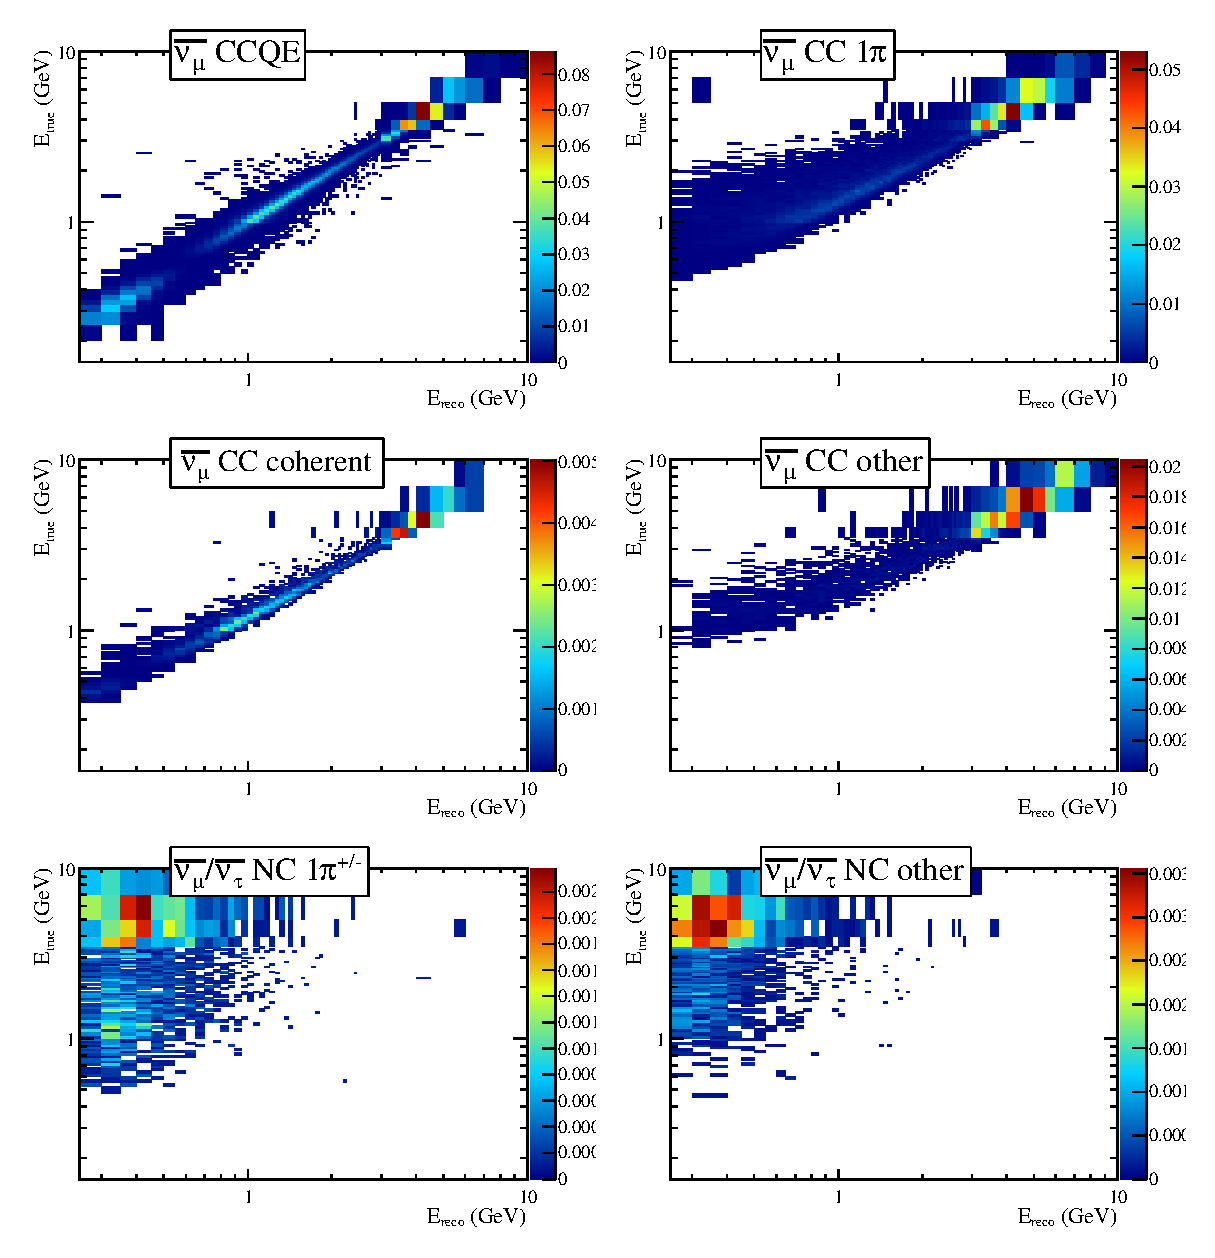
\includegraphics[width=35pc]{../images/templates/mc_template_2}
\caption{
  Nominal ($E_{t}$, $E_{r}$) 1-ring $\mu$-like MC templates. 
  The templates are shown for
  $\bar{\nu_{\mu}}$ CCQE, 
  $\bar{\nu_{\mu}}$ CC1$\pi$, 
  $\bar{\nu_{\mu}}$ CC coherent, 
  $\bar{\nu_{\mu}}$ CC other, 
  $\bar{\nu_{\mu}}$ NC1$\pi^{\pm}$, 
  $\bar{\nu_{\mu}}$ NC other.
}
\label{fig:etrue_ereco_templates:numubar}
\end{figure*}

\begin{figure*}[htb]
\center
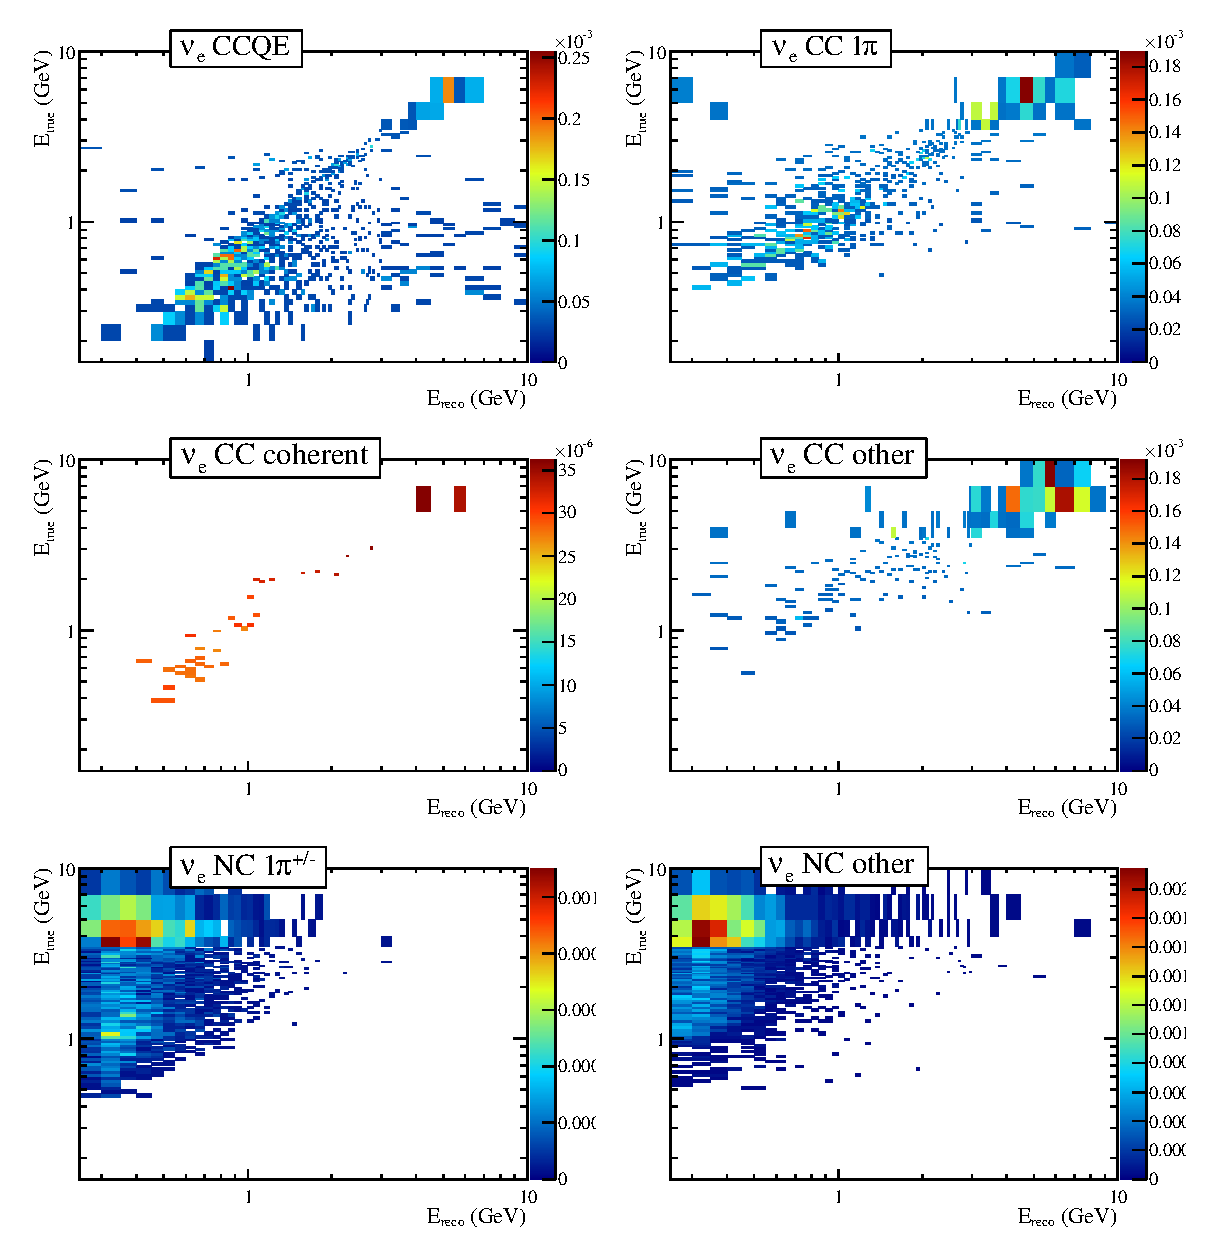
\includegraphics[width=35pc]{../images/templates/mc_template_3}
\caption{
  Nominal ($E_{t}$, $E_{r}$) 1-ring $\mu$-like MC templates. 
  The templates are shown for
  $\nu_{e}$ CCQE, 
  $\nu_{e}$ CC1$\pi$,
  $\nu_{e}$ CC coherent,
  $\nu_{e}$ CC other,
  $\nu_{e}$ NC1$\pi^{\pm}$,
  $\nu_{e}$ NC other.
}
\label{fig:etrue_ereco_templates:nue}
\end{figure*}

\begin{figure*}[htb]
\center
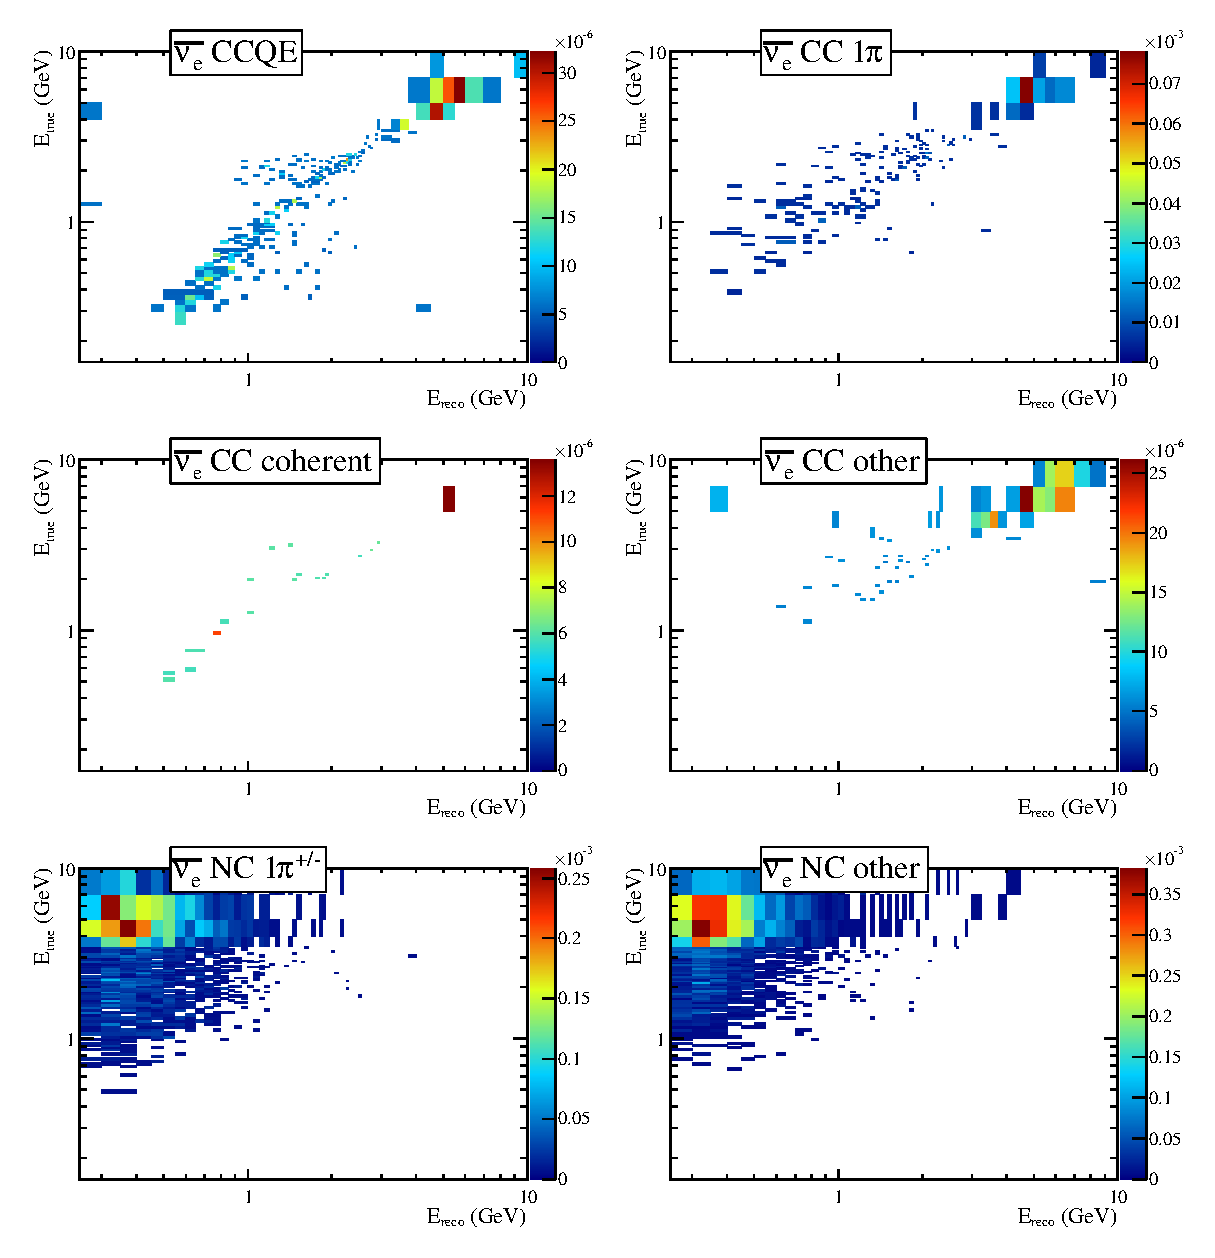
\includegraphics[width=35pc]{../images/templates/mc_template_4}
\caption{
  Nominal ($E_{t}$, $E_{r}$) 1-ring $\mu$-like MC templates. 
  The templates are shown for
  $\bar{\nu_{e}}$ CCQE, 
  $\bar{\nu_{e}}$ CC1$\pi$,
  $\bar{\nu_{e}}$ CC coherent,
  $\bar{\nu_{e}}$ CC other,
  $\bar{\nu_{e}}$ NC1$\pi^{\pm}$,
  $\bar{\nu_{e}}$ NC other.
}
\label{fig:etrue_ereco_templates:nuebar}
\end{figure*}

\begin{figure*}[htb]
\center
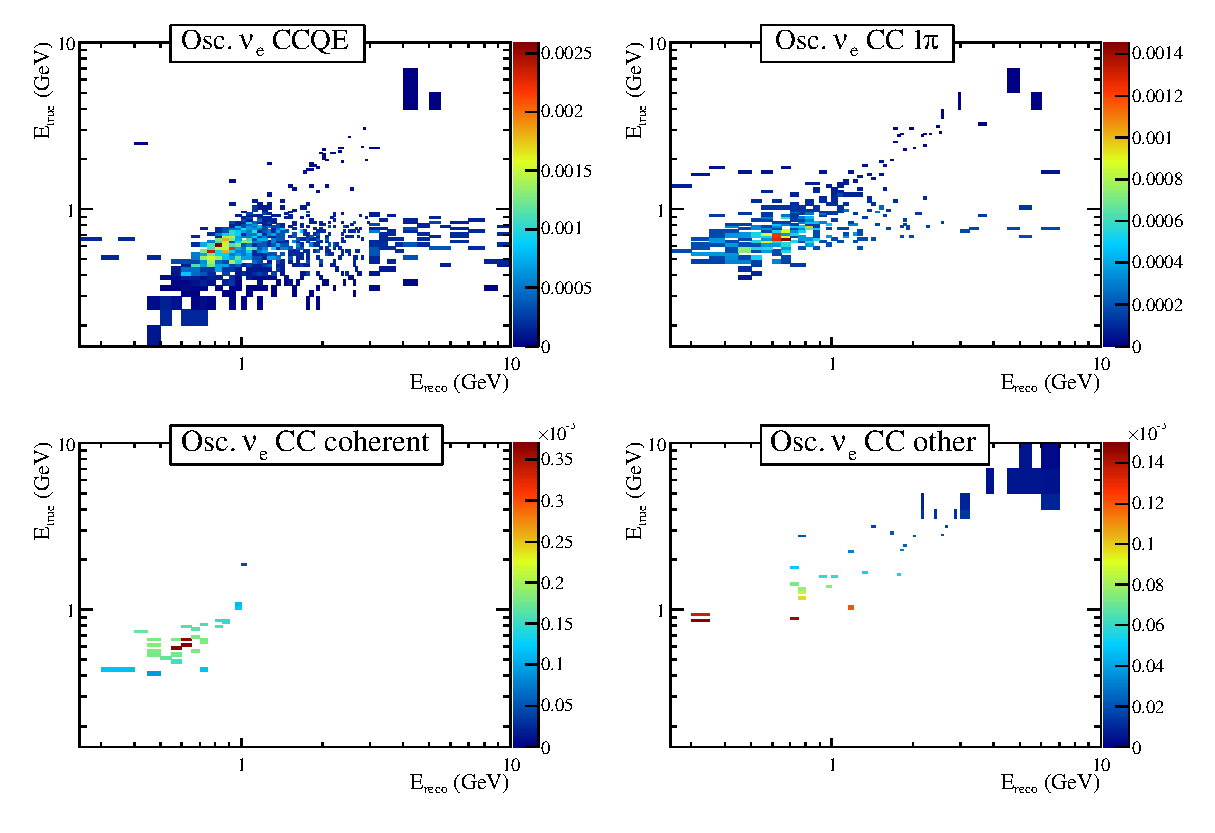
\includegraphics[width=35pc]{../images/templates/mc_template_5}
\caption{
  Nominal ($E_{t}$, $E_{r}$) 1-ring $\mu$-like MC templates. 
  The templates are shown for
  osc. $\nu_{e}$ CCQE, 
  osc. $\nu_{e}$ CC1$\pi$,
  osc. $\nu_{e}$ CC coherent and
  osc. $\nu_{e}$ CC other.
}
\label{fig:etrue_ereco_templates:oscnue}
\end{figure*}

